%=====================================================================
%  UpDesk — B.Tech / M.Tech Project Report
%  Madan Mohan Malaviya University of Technology, Gorakhpur
%  Compile with: pdfLaTeX  (Overleaf: Menu -> Compiler -> pdfLaTeX)
%=====================================================================
\documentclass[12pt,a4paper,oneside]{report}

%----------------------- Page geometry -------------------------------
\usepackage[a4paper,left=1.5in,right=1in,top=1in,bottom=1in]{geometry}

%----------------------- Fonts & encoding ----------------------------
\usepackage[T1]{fontenc}
\usepackage[utf8]{inputenc}
\usepackage{times}                 % Times New Roman look
\usepackage{setspace}
\onehalfspacing                    % use \doublespacing if your dept. asks

%----------------------- Graphics, tables, code ----------------------
\usepackage{graphicx}
\graphicspath{{figures/}}
\usepackage{booktabs}
\usepackage{longtable}
\usepackage{multirow}
\usepackage{array}
\usepackage{float}
\usepackage{listings}
\usepackage{xcolor}
\usepackage{amsmath,amssymb}
\usepackage{tikz}
\usetikzlibrary{arrows.meta,positioning,shapes.geometric,fit,calc}

%----------------------- Headings ------------------------------------
\usepackage{titlesec}
\titleformat{\chapter}[display]
  {\normalfont\bfseries\centering}
  {\Large CHAPTER \thechapter}{6pt}{\Large\MakeUppercase}
\titlespacing*{\chapter}{0pt}{-20pt}{24pt}
\titleformat{\section}{\normalfont\bfseries\large}{\thesection}{1em}{}
\titleformat{\subsection}{\normalfont\bfseries\normalsize}{\thesubsection}{1em}{}

%----------------------- Headers/footers -----------------------------
\usepackage{fancyhdr}
\pagestyle{fancy}
\fancyhf{}
\fancyfoot[C]{\thepage}
\renewcommand{\headrulewidth}{0pt}
\fancypagestyle{plain}{\fancyhf{}\fancyfoot[C]{\thepage}\renewcommand{\headrulewidth}{0pt}}

%----------------------- Links & captions ----------------------------
\usepackage{caption}
\captionsetup{font=small,labelfont=bf,justification=centering}
\usepackage[hidelinks]{hyperref}

%----------------------- Code listing style --------------------------
\definecolor{codegray}{gray}{0.95}
\definecolor{codekw}{RGB}{0,0,180}
\definecolor{codecmt}{RGB}{0,120,0}
\definecolor{codestr}{RGB}{170,0,60}
\lstdefinestyle{updesk}{
  backgroundcolor=\color{codegray},
  basicstyle=\ttfamily\footnotesize,
  keywordstyle=\color{codekw}\bfseries,
  commentstyle=\color{codecmt}\itshape,
  stringstyle=\color{codestr},
  breaklines=true,
  captionpos=b,
  frame=single,
  numbers=left,
  numberstyle=\tiny,
  numbersep=8pt,
  showstringspaces=false,
  tabsize=2
}
\lstset{style=updesk}
\lstdefinelanguage{Rust}{
  keywords={as,async,await,break,const,continue,crate,dyn,else,enum,extern,false,fn,for,if,impl,in,let,loop,match,mod,move,mut,pub,ref,return,self,Self,static,struct,super,trait,true,type,unsafe,use,where,while},
  keywordstyle=\color{codekw}\bfseries,
  ndkeywords={String,Vec,Option,Result,Some,None,Ok,Err,u8,u32,u64,i32,usize,bool},
  sensitive=true,
  comment=[l]{//},
  morecomment=[s]{/*}{*/},
  morestring=[b]"
}

%----------------------- Handy macros --------------------------------
\newcommand{\updesk}{UpDesk}
\newcommand{\figref}[1]{Fig.~\ref{#1}}
\newcommand{\tabref}[1]{Table~\ref{#1}}

%=====================================================================
\begin{document}

%------------------------ FRONT MATTER -------------------------------
\pagenumbering{roman}

\begin{titlepage}
\thispagestyle{empty}
\begin{center}

{\Large\bfseries UPDESK: A SECURE PEER-TO-PEER REMOTE\\[4pt]
DESKTOP SYSTEM WITH AN UNATTENDED\\[4pt]
NATIVE HOST}\\[28pt]

{\large A Project Report}\\[10pt]
{\normalsize Submitted\\
In Partial Fulfillment of the Requirements\\
For the Award of the Degree of}\\[10pt]

{\large\bfseries Bachelor of Technology}\\[6pt]
{\normalsize in}\\[6pt]
{\large\bfseries Computer Science and Engineering}\\[24pt]

{\normalsize \textit{By}}\\[8pt]
{\large\bfseries NIKHIL SRIVASTAVA}\\[4pt]
{\normalsize (Roll No.\ \rule{2.2cm}{0.4pt})}\\[24pt]

{\normalsize \textit{Under the Supervision of}}\\[8pt]
{\large\bfseries \rule{5cm}{0.4pt}}\\[2pt]
{\normalsize (Associate Professor)}\\[28pt]

\IfFileExists{figures/mmmut_logo.png}
  {\includegraphics[width=0.22\textwidth]{mmmut_logo}\\[16pt]}
  {\rule{0.22\textwidth}{0.22\textwidth}\\[6pt]{\scriptsize[ Replace with figures/mmmut\_logo.png ]}\\[16pt]}

{\normalsize\bfseries DEPARTMENT OF COMPUTER SCIENCE AND ENGINEERING}\\[4pt]
{\normalsize\bfseries MADAN MOHAN MALAVIYA UNIVERSITY OF TECHNOLOGY}\\[4pt]
{\normalsize\bfseries GORAKHPUR-273010 (UP, INDIA)}\\[16pt]
{\normalsize July, 2026}

\end{center}
\end{titlepage}

\thispagestyle{empty}
\vspace*{\fill}
\begin{center}
\copyright\ M.M.M. University of Technology, Gorakhpur, (U.P.)-273010, INDIA\\[6pt]
ALL RIGHTS RESERVED
\end{center}
\vspace*{\fill}
\clearpage

\chapter*{Candidate's Declaration}
\addcontentsline{toc}{chapter}{Candidate's Declaration}
\thispagestyle{plain}

I declare that this written submission represents my work and ideas in my own
words and where others' ideas or words have been included, I have adequately
cited and referenced the original sources. I also declare that I have adhered to
all principles of academic honesty and integrity and have not misrepresented or
fabricated or falsified any idea, data, fact or source in my submission. I
understand that any violation of the above will be a cause for disciplinary
action by the University and can also evoke penal action from the sources which
have thus not been properly cited or from whom proper permission has not been
taken when needed.

\vspace{2.2cm}
\noindent\rule{7cm}{0.4pt}\\
(Signature)

\vspace{0.8cm}
\noindent\rule{7cm}{0.4pt}\\
(Name of the Student)

\vspace{0.8cm}
\noindent\rule{7cm}{0.4pt}\\
(Roll No.)

\vspace{0.8cm}
\noindent\rule{7cm}{0.4pt}\\
(Name of Department)

\vspace{1.2cm}
\noindent Date: \rule{4cm}{0.4pt}

\clearpage

\chapter*{Certificate}
\addcontentsline{toc}{chapter}{Certificate}
\thispagestyle{plain}

This is to certify that \textbf{Nikhil Srivastava} has carried out the project
work presented in this report entitled \textbf{``UpDesk: A Secure Peer-to-Peer
Remote Desktop System with an Unattended Native Host''} for the award of the
degree of Bachelor of Technology in Computer Science and Engineering from Madan
Mohan Malaviya University of Technology, Gorakhpur, under my supervision. The
report embodies the result of original work and studies carried out by the
student himself and the contents of the report do not form the basis for the
award of any other degree to the candidate or to anybody else.

\vspace{3cm}
\begin{flushright}
\noindent\rule{7cm}{0.4pt}\\
Signature of Supervisor\\
Name: \rule{4.5cm}{0.4pt}\\
Department of Computer Science and Engineering\\
M.\,M.\,M. University of Technology, Gorakhpur\\[10pt]
Date: \rule{4cm}{0.4pt}
\end{flushright}

\clearpage

\chapter*{Acknowledgement}
\addcontentsline{toc}{chapter}{Acknowledgement}
\thispagestyle{plain}

I wish to record my sincere gratitude to my supervisor for the patience,
technical direction and steady encouragement extended to me throughout this
work. The freedom to attempt an unconventional design, together with timely
correction whenever the approach drifted, shaped this project far more than any
single technical decision recorded in these pages.

I am thankful to the Head of the Department and to the faculty members of the
Department of Computer Science and Engineering, Madan Mohan Malaviya University
of Technology, Gorakhpur, for providing the laboratory facilities and the
academic environment in which this system could be built and tested. Access to a
second physical machine on the departmental network was essential for validating
the two-host scenarios described in Chapter~6, and I acknowledge that support
with thanks.

I also record my appreciation of the maintainers of the open-source projects on
which this work stands --- notably the Rust asynchronous ecosystem, the
\texttt{webrtc-rs} stack and the Tauri application framework. A defect I
encountered in DTLS curve negotiation was resolved by studying their source
directly, and that would not have been possible with closed software.

Finally, I thank my family and friends for their constant support during the
long debugging sessions that a systems project of this nature inevitably
demands.

\vspace{2cm}
\begin{flushright}
\textbf{Nikhil Srivastava}
\end{flushright}

\clearpage

\chapter*{Abstract}
\addcontentsline{toc}{chapter}{Abstract}
\thispagestyle{plain}

Remote desktop access has become ordinary infrastructure for technical support,
distributed teams and unattended server administration. The tools in common use,
however, force an uncomfortable choice. Products such as TeamViewer and AnyDesk
are convenient but proprietary, and every session is mediated by vendor
infrastructure the user cannot inspect. Protocol-level alternatives such as VNC
and Microsoft RDP are open or well-documented but assume direct network
reachability, which is rarely available between two machines that both sit
behind network address translation.

This project presents \textbf{UpDesk}, a remote desktop system implemented
predominantly in Rust that addresses both concerns at once. Media and control
data travel over a direct WebRTC peer connection established between the
controlling and controlled machines, so screen frames never pass through a
central server in the common case. A small signaling server participates only
during connection establishment: it authenticates each endpoint using an
Ed25519 challenge--response handshake, relays session-description and ICE
candidate messages, and then steps aside. Because the server never possesses the
DTLS-SRTP keys negotiated by the peers, it cannot decrypt the stream it helped
to arrange.

The second contribution of the work is an \emph{unattended native host}. A
conventional web-technology host is constrained by the browser security model:
screen capture through \texttt{getDisplayMedia} demands a user gesture and a
picker dialogue, and it cannot observe the Windows login screen or User Account
Control prompts, which are rendered on an isolated secure desktop. UpDesk
therefore adds a standalone Rust binary that captures the framebuffer directly,
encodes it to H.264, publishes it on a native WebRTC track, and injects keyboard
and pointer events back into the active desktop. Registered as a Windows
service, this binary is available from boot and before any user has logged in.

The system was evaluated on a two-machine local network and across the public
Internet. Direct peer connectivity was achieved in the tested NAT
configurations, end-to-end latency remained in the range appropriate for
interactive use at 1080p, and the service-mode host survived reboot and session
switching without operator intervention. The report documents the protocol
design, the cryptographic reasoning behind it, the implementation of each
subsystem, and the measurements obtained.

\vspace{0.6cm}
\noindent\textbf{Keywords:} Remote Desktop, WebRTC, Peer-to-Peer, NAT Traversal,
Ed25519, Rust, Screen Capture, Windows Service, Tauri.

\clearpage


\tableofcontents
\clearpage
\listoffigures
\clearpage
\listoftables
\clearpage
\chapter*{List of Abbreviations}
\addcontentsline{toc}{chapter}{List of Abbreviations}
\thispagestyle{plain}

\begin{longtable}{@{}p{3.2cm}p{10.5cm}@{}}
\toprule
\textbf{Abbreviation} & \textbf{Expansion} \\
\midrule
\endhead
API    & Application Programming Interface \\
DTLS   & Datagram Transport Layer Security \\
DXGI   & DirectX Graphics Infrastructure \\
ECDHE  & Elliptic Curve Diffie--Hellman Ephemeral \\
GUI    & Graphical User Interface \\
ICE    & Interactive Connectivity Establishment \\
IPC    & Inter-Process Communication \\
JSON   & JavaScript Object Notation \\
NAT    & Network Address Translation \\
P2P    & Peer-to-Peer \\
RDP    & Remote Desktop Protocol \\
RTT    & Round-Trip Time \\
SDP    & Session Description Protocol \\
SRTP   & Secure Real-time Transport Protocol \\
STUN   & Session Traversal Utilities for NAT \\
TLS    & Transport Layer Security \\
TURN   & Traversal Using Relays around NAT \\
UAC    & User Account Control \\
VNC    & Virtual Network Computing \\
WSS    & WebSocket Secure \\
\bottomrule
\end{longtable}

\clearpage


%------------------------ MAIN MATTER --------------------------------
\clearpage
\pagenumbering{arabic}

\chapter{Introduction}

The ability to operate a computer that is physically somewhere else has moved
from a specialist convenience to an assumed capability. A support engineer
expects to reach a customer's laptop without travelling to it; an administrator
expects to reach a rack-mounted server that has no monitor attached; a student
expects to reach the laboratory machine that holds a licensed toolchain. Each of
these situations is served today, but rarely by the same tool and rarely without
a compromise the user is asked to accept silently.

This chapter states the motivation for building a new remote desktop system,
defines the problem precisely, lists the objectives that guided the design, and
outlines how the remainder of the report is organised.

\section{Overview}

A remote desktop system performs three tasks continuously and must perform all
three well. It \emph{captures} the visual state of the controlled machine, it
\emph{transports} that state to the controlling machine, and it \emph{returns}
keyboard and pointer events in the opposite direction. The difficulty is that
these tasks pull against one another. Capturing at high fidelity produces more
data than a residential uplink can carry; compressing aggressively introduces
delay that makes the pointer feel detached from the hand; and transporting
anything at all requires that two machines which may both be hidden behind
network address translation somehow find a path to each other.

Existing systems resolve this tension in different places. Microsoft's Remote
Desktop Protocol achieves excellent efficiency by transmitting drawing
primitives rather than pixels, but it is tied to the Windows display stack and
assumes a routable address or a corporate gateway. Virtual Network Computing
transmits framebuffer rectangles and is admirably portable, but it was designed
for local networks and its bandwidth behaviour on a wide-area link is poor.
Commercial products such as TeamViewer and AnyDesk solve reachability elegantly
by routing every session through vendor-operated relays, and in doing so place
the vendor in a position of complete visibility over traffic the user may regard
as sensitive.

\updesk{} takes the position that the reachability problem and the trust problem
are separable. Reachability is a well-studied networking question with a
standard answer --- the ICE framework, with STUN for address discovery and TURN
as a fallback relay. Trust is a cryptographic question, and the answer is to
ensure that whatever infrastructure assists with reachability is structurally
incapable of reading the session. WebRTC provides both: ICE for connectivity and
mandatory DTLS-SRTP for media encryption, with keys negotiated directly between
the endpoints. A signaling server is still required to introduce the peers, but
it handles only metadata.

\section{Motivation}

Three observations motivated this work.

\textbf{Relay-mediated architectures concentrate risk.} When every frame of a
support session traverses a third party's servers, the confidentiality of that
session rests entirely on the operator's policy and competence rather than on
mathematics. A design in which the coordinating server never holds a media key
removes that dependence. This is not a hypothetical concern for an
administrator entering credentials on a remote machine during a support call.

\textbf{Unattended access is where most remote desktop tools quietly fail.} A
system that requires a human at the far end to click ``accept'' is adequate for
support but useless for the server in the corner that needs attention at two in
the morning. Genuine unattended operation requires the host to run before any
user logs in, to survive reboots, and to remain usable while Windows displays
its login screen or a User Account Control prompt. Those screens are drawn on a
separate, isolated desktop that an ordinary user-session application cannot
capture. Meeting this requirement is a systems problem, not a user-interface
problem, and it drove much of the architecture described in Chapter~4.

\textbf{Systems languages have become practical for this class of software.}
Remote desktop hosts handle untrusted network input while manipulating raw
framebuffers --- historically a rich source of memory-safety vulnerabilities.
Rust offers memory safety without a garbage collector, and its asynchronous
ecosystem is now mature enough to implement WebRTC, TLS termination and video
encoding in one coherent codebase. Building \updesk{} predominantly in Rust was
therefore both an engineering and a security decision.

\section{Problem Statement}

\emph{To design and implement a cross-platform remote desktop system in which
screen and control data travel over a directly negotiated, end-to-end encrypted
peer-to-peer channel; in which the coordinating server authenticates endpoints
cryptographically but cannot decrypt session content; and which additionally
provides a fully unattended host capable of operating from system boot,
including on privileged desktops that conventional user-session applications
cannot capture.}

\section{Objectives}

The work was directed at the following objectives.

\begin{enumerate}
  \item To design a signaling protocol that authenticates hosts and controllers
        using Ed25519 public-key cryptography, resists replay through a
        challenge--response exchange, and exposes no session content to the
        server.
  \item To implement that signaling server in Rust with optional TLS termination
        and optional persistence of enrolled identities and session audit
        records.
  \item To implement a graphical host application and a graphical controller
        application that establish a WebRTC peer connection, stream video in one
        direction and control events in the other.
  \item To implement a headless native host that captures the framebuffer
        without any user gesture, encodes it to H.264, and serves it over a
        native WebRTC peer connection.
  \item To implement native keyboard and pointer injection so that the native
        host supports control and not merely observation.
  \item To package the native host as a Windows service so that it is present
        from boot, survives reboot and session switching, and can reach the
        active desktop.
  \item To evaluate the resulting system for connection-establishment success
        across NAT configurations, interactive latency, frame rate and bandwidth
        consumption.
\end{enumerate}

\section{Scope and Limitations}

The implementation targets Windows as the host platform, because the unattended
and secure-desktop requirements are inherently platform-specific and Windows
presents the hardest version of that problem. The controller application is
portable, and exploratory Android clients exist in the repository but are not
claimed as completed contributions. Audio forwarding and file transfer were
deliberately excluded in order to keep the video and control paths correct
before adding surface area. Multi-monitor capture is limited to the primary
display. These boundaries are revisited in Chapter~7 as directions for further
work.

\section{Organisation of the Report}

Chapter~2 surveys existing remote desktop protocols and products and the
underlying real-time communication technologies, and identifies the gap this
work addresses. Chapter~3 records the functional, non-functional and
environmental requirements. Chapter~4 presents the system architecture: the
component decomposition, the signaling protocol, the connection-establishment
sequence, and the security model. Chapter~5 describes the implementation of each
subsystem with reference to the actual codebase. Chapter~6 reports the
experimental setup and the measurements obtained. Chapter~7 concludes and
proposes future work.

\chapter{Literature Review}

This chapter examines the protocols, products and enabling technologies that
define the current state of remote desktop access, and closes by identifying the
gap that \updesk{} occupies.

\section{Remote Framebuffer and VNC}

Virtual Network Computing, developed at the Olivetti Research Laboratory and
standardised as the Remote Framebuffer protocol in RFC~6143, is the conceptual
ancestor of most open remote desktop software. Its model is deliberately thin:
the server exports a rectangular framebuffer, the client requests updates, and
the server responds with rectangles that have changed, optionally encoded using
schemes such as Hextile, ZRLE or Tight.

The strength of this design is portability. Because the protocol reasons about
pixels rather than drawing commands, a VNC server can be written for any system
that can read its own screen. The corresponding weakness is efficiency. Video
playback or window dragging invalidates large regions, and rectangle-oriented
encodings degrade badly under such motion. RFB also assumes the client can open
a TCP connection to the server, which on the modern Internet is usually false
without manual port forwarding. Security was not part of the original design;
encryption is provided, when at all, by tunnelling or by vendor extensions.

\section{Microsoft Remote Desktop Protocol}

RDP takes the opposite approach. Rather than shipping pixels, it intercepts
drawing operations and transmits high-level primitives --- glyphs, blits,
geometric fills --- which the client replays locally. For conventional desktop
work this is dramatically more efficient than any framebuffer encoding, and
successive revisions have added RemoteFX and H.264 codecs for content that does
not decompose into primitives.

RDP is mature, well integrated with Windows session management, and capable of
reaching the login screen because it is part of the operating system rather than
an application running inside a session. Its limitations for the present purpose
are that it is tightly coupled to the Windows display architecture, that its
implementation is closed, and that reaching an RDP host from outside a network
requires either a routable address, a virtual private network, or a Remote
Desktop Gateway. Exposing RDP directly to the Internet is widely documented as a
significant risk and is a common initial vector for ransomware intrusion.

\section{Commercial Peer-Assisted Products}

TeamViewer, AnyDesk and similar commercial tools solved the reachability problem
in the way users actually experience it: the host registers with vendor
infrastructure and is addressed by a short numeric identifier, and the vendor
arranges connectivity irrespective of NAT. AnyDesk's DeskRT codec, in
particular, is specialised for graphical user interface content and achieves
notably low latency.

These products are highly capable, and their user experience informed the design
of \updesk{}'s connect-identifier scheme. The architectural objection is one of
trust rather than quality. Session traffic is arranged, and frequently relayed,
by infrastructure the user neither controls nor can audit, and the identifier
namespace itself is vendor-operated. Published incidents in which support
sessions were abused illustrate that the concentration of capability is a real
consideration and not merely a theoretical one.

\section{RustDesk and the Open Alternative}

RustDesk is an open-source remote desktop implementation written in Rust that
mirrors the commercial user experience --- numeric identifiers, self-hostable
relay and rendezvous servers --- while permitting inspection of the source. Its
architecture separates a native capture library from a service component, which
is precisely the structure required to reach privileged desktops on Windows.

RustDesk is the closest prior work to this project and was studied carefully
during design. \updesk{} differs in two respects that are relevant to the
contribution claimed here. First, it uses standard WebRTC as its transport, so
media encryption, congestion control and ICE behaviour are inherited from a
widely reviewed implementation rather than from a bespoke protocol. Second, its
signaling layer authenticates every endpoint with an Ed25519
challenge--response, with enrollment gated by one-time codes, making device
identity a first-class element of the protocol rather than a property of a
shared password.

\section{WebRTC as a Transport}

WebRTC is a set of standards for real-time communication between peers,
comprising media capture, a peer connection abstraction, and data channels. Its
relevance here rests on three properties.

\textbf{Connectivity.} Interactive Connectivity Establishment (RFC~8445) has
each peer gather candidate transport addresses --- host addresses, server-
reflexive addresses discovered through STUN, and relayed addresses obtained from
TURN --- exchange them, and probe candidate pairs systematically until a
working path is found. This resolves the NAT traversal problem that defeats VNC
and RDP without operator configuration.

\textbf{Security.} Media encryption is not optional. Peers perform a DTLS
handshake and derive SRTP keys from it, so the payload is protected end to end.
A signaling server that only relays session descriptions and candidates cannot
recover those keys, which is exactly the property \updesk{} requires.

\textbf{Adaptivity.} The stack includes congestion control, packet loss
concealment and jitter buffering developed for conferencing traffic, which
transfers directly to screen streaming.

WebRTC deliberately does not specify signaling. Peers must exchange SDP offers,
answers and ICE candidates over some out-of-band channel of the application's
choosing, and the design of that channel is where an application's security
model is largely decided.

\section{Screen Capture on Windows}

Three mechanisms are relevant. The \texttt{getDisplayMedia} API available to web
content is simple and cross-platform, but the browser security model requires a
user gesture and a source-selection dialogue, and content on the secure desktop
is never visible to it. The Desktop Duplication API exposed through DXGI
provides efficient access to the composited desktop surface with damage regions,
and is the basis of most native Windows capture. The newer
Windows.Graphics.Capture API offers per-window capture with a cleaner interface
at the cost of requiring recent Windows versions.

Critically, none of these can observe the Winlogon secure desktop from an
ordinary user session. Windows isolates the login screen and UAC prompts on a
separate desktop in a distinct session precisely to prevent one application from
observing or driving another's credential entry. Reaching it requires a process
running as SYSTEM that can attach to the active desktop --- which is why the
architecture in Chapter~4 includes a service component.

\section{Identified Gap}

The survey suggests the following. Open protocols such as RFB and RDP are
transparent but assume reachability that ordinary networks do not provide.
Commercial products provide reachability but require trust in infrastructure
that cannot be audited. RustDesk narrows the gap substantially but implements
its own transport and its own security layer. There remains room for a system
that (i) uses standard, widely reviewed WebRTC for transport and encryption,
(ii) authenticates endpoints with public-key identity so that the signaling
server can verify who is connecting without being able to read what is sent, and
(iii) treats unattended, pre-login, secure-desktop-capable operation as a design
requirement rather than an afterthought. \updesk{} is an attempt to occupy that
position.

\tabref{tab:comparison} summarises the comparison.

\begin{table}[H]
\centering
\caption{Comparison of remote desktop approaches}
\label{tab:comparison}
\small
\begin{tabular}{@{}lccccc@{}}
\toprule
\textbf{System} & \textbf{Open} & \textbf{NAT} & \textbf{E2E} & \textbf{Pre-login} & \textbf{Transport} \\
 & & \textbf{traversal} & \textbf{encrypted} & \textbf{access} & \\
\midrule
VNC (RFB)   & Yes & No      & Optional & No  & TCP \\
RDP         & No  & Gateway & Yes      & Yes & TCP/UDP \\
TeamViewer  & No  & Yes     & Claimed  & Yes & Proprietary \\
AnyDesk     & No  & Yes     & Claimed  & Yes & Proprietary \\
RustDesk    & Yes & Yes     & Yes      & Yes & Custom \\
\textbf{UpDesk} & Yes & Yes & Yes      & Yes & WebRTC \\
\bottomrule
\end{tabular}
\end{table}

\chapter{Requirement Analysis}

This chapter records the requirements that the system was built to satisfy,
separated into functional behaviour, quality attributes, and the environment
assumed by the implementation.

\section{Functional Requirements}

\tabref{tab:funcreq} lists the functional requirements, each with the
identifier used elsewhere in the report.

\begin{table}[H]
\centering
\caption{Functional requirements}
\label{tab:funcreq}
\small
\begin{tabular}{@{}p{1.4cm}p{8.4cm}p{2.6cm}@{}}
\toprule
\textbf{ID} & \textbf{Requirement} & \textbf{Priority} \\
\midrule
FR-1 & A device or controller shall enroll using a single-use code and thereafter be identified by an Ed25519 public key. & Essential \\
FR-2 & The signaling server shall authenticate every connection by a challenge--response signature before accepting any other message. & Essential \\
FR-3 & A host shall register its availability and be addressable by a nine-digit connect identifier. & Essential \\
FR-4 & A controller shall initiate a session by connect identifier and the host shall be able to accept or reject it. & Essential \\
FR-5 & The peers shall exchange SDP offers, answers and ICE candidates through the signaling server and establish a direct peer connection. & Essential \\
FR-6 & The host shall capture the primary display and transmit it as an encoded video stream. & Essential \\
FR-7 & The controller shall transmit keyboard and pointer events, which the host shall inject into the local input queue. & Essential \\
FR-8 & The native host shall operate with no window, no user gesture and no source picker. & Essential \\
FR-9 & The native host shall accept unattended sessions automatically on presentation of a configured password. & Essential \\
FR-10 & The native host shall install as a Windows service, start at boot and survive session switching. & Essential \\
FR-11 & The signaling server shall optionally persist enrolled identities and a session audit log to PostgreSQL. & Desirable \\
FR-12 & The signaling server shall optionally terminate TLS and serve \texttt{wss://}. & Desirable \\
FR-13 & An administrative utility shall list enrolled devices with their connect identifiers. & Desirable \\
\bottomrule
\end{tabular}
\end{table}

\section{Non-Functional Requirements}

\subsection{Performance}

Interactive remote control is unusable if the delay between an input event and
the corresponding visual change is perceptible as lag. The target adopted was an
end-to-end glass-to-glass latency below 150\,ms on a local network and below
250\,ms over a typical broadband path, with a sustained frame rate of at least
25\,frames per second at 1920$\times$1080. Bandwidth consumption was to remain
within the capability of an ordinary residential uplink for typical desktop
content.

\subsection{Security}

The signaling server must not be able to decrypt session media. Endpoint
identity must rest on private keys that never leave the machine holding them.
Enrollment must not be open: possession of a valid one-time code is required
before a key is accepted. Unattended acceptance must be gated by a secret that
is verified by the host rather than by the server.

\subsection{Reliability and Availability}

The service-mode host must return to service automatically after a reboot,
after a user logs off, and after the console session is switched. Failure of the
signaling server must not terminate sessions that have already established a
direct peer connection, since the server is not on the media path.

\subsection{Maintainability}

The system is organised as a Cargo workspace with separate crates for the
signaling server, the native host and the service supervisor, so that each can
be built and tested in isolation. Protocol messages are JSON, which keeps them
inspectable during development.

\section{Hardware and Software Environment}

\begin{table}[H]
\centering
\caption{Development and test environment}
\label{tab:env}
\small
\begin{tabular}{@{}p{4.2cm}p{9cm}@{}}
\toprule
\textbf{Component} & \textbf{Specification} \\
\midrule
Host machine        & Windows 11 Pro (build 26200), x86-64, 16\,GB RAM \\
Controller machine  & Windows 11, x86-64, 8\,GB RAM \\
Language toolchain  & Rust (2021 edition), stable channel \\
Async runtime       & Tokio \\
WebRTC stack        & \texttt{webrtc-rs} 0.11, with a patched \texttt{webrtc-dtls} \\
Video encoder       & OpenH264 via the \texttt{openh264} crate \\
Screen capture      & \texttt{scrap} (Desktop Duplication) \\
Input injection     & \texttt{enigo}, and the Win32 \texttt{SendInput} path \\
Signaling transport & \texttt{tokio-tungstenite} over WebSocket / WSS \\
Cryptography        & \texttt{ed25519-dalek} 2.x \\
TLS                 & \texttt{tokio-rustls} with the \texttt{ring} provider \\
Persistence         & PostgreSQL via \texttt{sqlx} (optional) \\
GUI applications    & Tauri with a WebView2 front end \\
Network             & 1\,Gbps switched LAN; consumer broadband with CGNAT for wide-area tests \\
\bottomrule
\end{tabular}
\end{table}

\section{Feasibility Study}

\textbf{Technical.} Every component has a viable Rust implementation, which was
confirmed by prototyping the riskiest element first --- silent framebuffer
capture --- before committing to the architecture. The one genuine technical
obstacle encountered was a DTLS handshake failure against current Chrome
versions, resolved as described in Section~5.6.

\textbf{Economic.} All dependencies are open source. The only recurring cost is
a modest virtual private server for signaling and an optional TURN relay, and
because media is peer-to-peer the relay is exercised only in the minority of
network configurations that defeat direct connectivity.

\textbf{Operational.} The host installs as a service with a single command and
requires no configuration beyond an enrollment code and an unattended password,
which is comparable to the deployment effort of the commercial alternatives.

\chapter{System Design}

This chapter presents the architecture of \updesk{}. It begins with the overall
component decomposition, then treats the signaling protocol, the
connection-establishment sequence, the data model and the security reasoning in
turn.

\section{Architectural Overview}

\updesk{} is composed of three cooperating roles and one coordinating service.
The \emph{controller} is the machine from which a user drives a remote session.
The \emph{host} is the machine being controlled; it exists in two forms, a
graphical Tauri application for attended use and a headless native binary for
unattended use. The \emph{signaling server} is a lightweight Rust process that
introduces controllers to hosts and relays the messages needed to negotiate a
peer connection, but carries no media. \figref{fig:arch} shows the arrangement.

\begin{figure}[H]
\centering
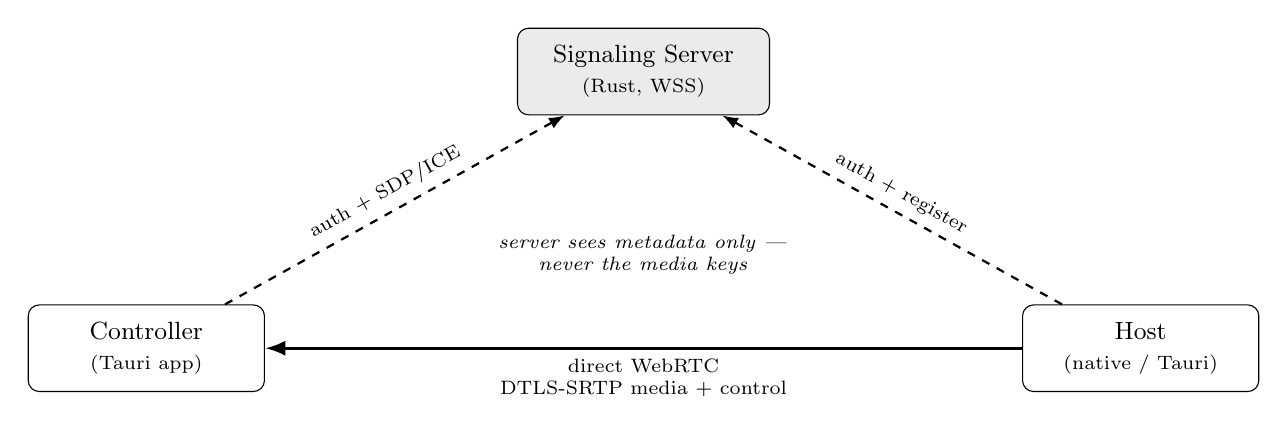
\begin{tikzpicture}[
  node distance=2.4cm and 3.2cm,
  box/.style={draw,rounded corners,minimum width=3cm,minimum height=1.1cm,align=center,font=\small},
  server/.style={draw,rounded corners,fill=black!8,minimum width=3.2cm,minimum height=1.1cm,align=center,font=\small},
  sig/.style={-{Latex[length=2mm]},dashed,thick},
  media/.style={-{Latex[length=2.6mm]},very thick}
]
  \node[server] (srv) {Signaling Server\\{\scriptsize (Rust, WSS)}};
  \node[box, below left=of srv] (ctl) {Controller\\{\scriptsize (Tauri app)}};
  \node[box, below right=of srv] (host) {Host\\{\scriptsize (native / Tauri)}};

  \draw[sig] (ctl) -- (srv) node[midway,above,sloped,font=\scriptsize] {auth + SDP/ICE};
  \draw[sig] (host) -- (srv) node[midway,above,sloped,font=\scriptsize] {auth + register};
  \draw[media] (host) -- (ctl)
      node[midway,below,font=\scriptsize,align=center] {direct WebRTC\\DTLS-SRTP media + control};

  \node[font=\scriptsize,align=center,below=1.4cm of srv] {\textit{server sees metadata only ---}\\\textit{never the media keys}};
\end{tikzpicture}
\caption{Component architecture. Dashed lines are signaling; the solid line is
the direct, end-to-end encrypted peer connection that carries screen frames and
control events.}
\label{fig:arch}
\end{figure}

The essential property visible in the figure is that the two solid endpoints
exchange media directly. The signaling server sits on the dashed paths only. It
authenticates both endpoints and passes their session descriptions back and
forth, but once the peer connection is live the server can be removed without
disturbing the session.

\section{The Native Host Internals}

The native host is the most involved component because it must do the work a
browser would otherwise do, without a browser. \figref{fig:nativehost} shows its
internal pipeline. A capture thread pulls framebuffers from the Desktop
Duplication API; each frame is handed to an H.264 encoder; encoded access units
are written onto a WebRTC video track; and, in the reverse direction, control
messages arriving on a data channel are decoded into synthetic input events and
injected into the desktop.

\begin{figure}[H]
\centering
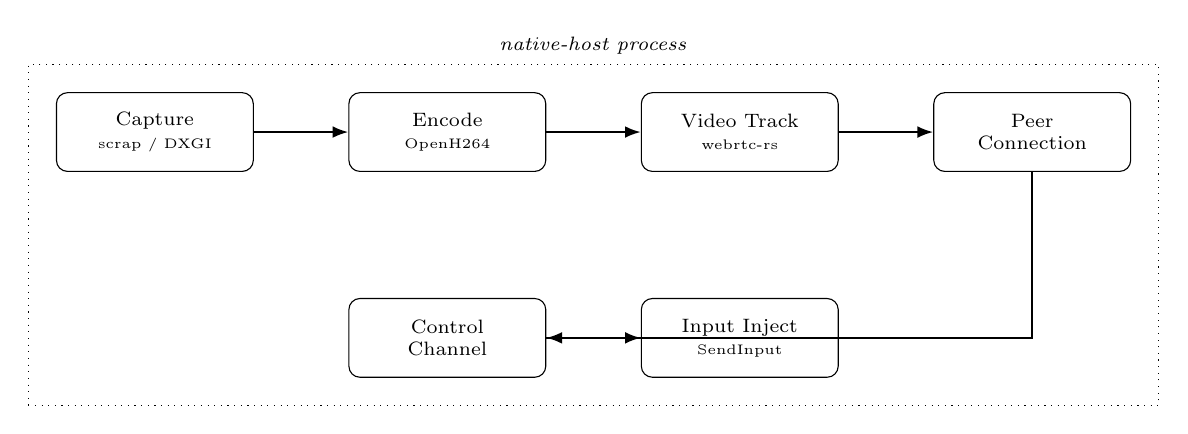
\begin{tikzpicture}[
  stage/.style={draw,rounded corners,minimum width=2.5cm,minimum height=1cm,align=center,font=\scriptsize},
  flow/.style={-{Latex[length=2mm]},thick},
  node distance=0.9cm and 1.2cm
]
  \node[stage] (cap) {Capture\\{\tiny scrap / DXGI}};
  \node[stage,right=of cap] (enc) {Encode\\{\tiny OpenH264}};
  \node[stage,right=of enc] (track) {Video Track\\{\tiny webrtc-rs}};
  \node[stage,right=of track] (pc) {Peer\\Connection};

  \node[stage,below=1.6cm of track] (inj) {Input Inject\\{\tiny SendInput}};
  \node[stage,left=of inj] (dc) {Control\\Channel};

  \draw[flow] (cap) -- (enc);
  \draw[flow] (enc) -- (track);
  \draw[flow] (track) -- (pc);
  \draw[flow] (pc.south) |- (dc);
  \draw[flow] (dc) -- (inj);

  \node[draw,dotted,fit=(cap)(enc)(track)(pc)(dc)(inj),inner sep=10pt,label={[font=\scriptsize]above:\textit{native-host process}}] {};
\end{tikzpicture}
\caption{Native host pipeline. The upper row is the outbound video path; the
lower row is the inbound control path.}
\label{fig:nativehost}
\end{figure}

\section{Signaling Protocol}

All signaling messages are JSON objects distinguished by a \texttt{type} field
and carried over a WebSocket (plain \texttt{ws://} in development,
\texttt{wss://} in deployment). \tabref{tab:messages} enumerates the message
types actually implemented by the server and the native host.

\begin{table}[H]
\centering
\caption{Signaling message types}
\label{tab:messages}
\small
\begin{tabular}{@{}p{3.2cm}p{2cm}p{7.6cm}@{}}
\toprule
\textbf{Message} & \textbf{Direction} & \textbf{Purpose} \\
\midrule
\texttt{auth\_init}      & server$\to$peer & Server issues a random challenge nonce. \\
\texttt{auth\_response}  & peer$\to$server & Peer returns its public key and an Ed25519 signature over the nonce. \\
\texttt{register}        & host$\to$server & Host announces availability under its connect identifier. \\
\texttt{connect\_request}& controller$\to$server & Controller asks to reach a host by connect identifier. \\
\texttt{session\_response}& host$\to$server & Host accepts or rejects the incoming request. \\
\texttt{offer}           & host$\to$controller & SDP offer, relayed by the server. \\
\texttt{answer}          & controller$\to$host & SDP answer, relayed by the server. \\
\texttt{ice\_candidate}  & both & An ICE candidate, relayed as it is discovered. \\
\texttt{end\_session}    & both & Orderly teardown of the signaling association. \\
\bottomrule
\end{tabular}
\end{table}

\subsection{Enrollment}

Before a machine can authenticate it must enroll. Enrollment is gated by a
single-use code of the form \texttt{DEV0-TEST:device} or
\texttt{CTL0-TEST:controller}, seeded in the server's configuration and consumed
on first use. During enrollment the peer generates an Ed25519 key pair, keeps
the private key locally, and registers the public key against the code. From
that point the public key \emph{is} the machine's identity; the code is spent
and cannot be reused. This deliberately prevents anonymous participation: an
attacker cannot register a host or controller without first obtaining a valid
code out of band.

\subsection{Authentication Handshake}

Every WebSocket connection begins with the same challenge--response exchange,
shown in \figref{fig:auth}, before any other message is honoured. The server
sends \texttt{auth\_init} carrying a fresh random nonce. The peer signs that
nonce with its Ed25519 private key and replies with \texttt{auth\_response}
containing its public key and the signature. The server verifies the signature
against the enrolled key. Because the nonce is random and single-use, a captured
\texttt{auth\_response} cannot be replayed against a later challenge.

\begin{figure}[H]
\centering
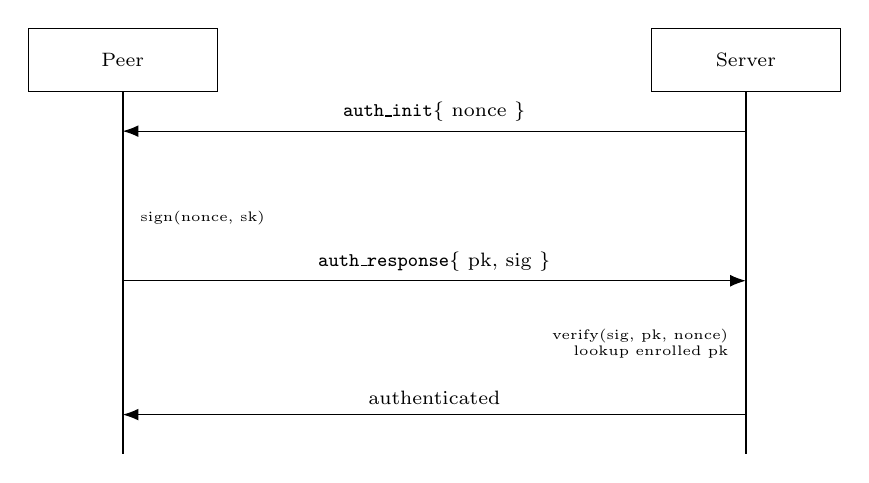
\begin{tikzpicture}[
  font=\scriptsize,
  actor/.style={draw,minimum width=2.4cm,minimum height=0.8cm},
  msg/.style={-{Latex[length=2mm]}}
]
  \node[actor] (p) {Peer};
  \node[actor,right=5.5cm of p] (s) {Server};
  \draw[thick] (p.south) -- ++(0,-4.6);
  \draw[thick] (s.south) -- ++(0,-4.6);
  \coordinate (p0) at ($(p.south)+(0,-0.5)$);
  \coordinate (s0) at ($(s.south)+(0,-0.5)$);
  \draw[msg] ($(s0)$) -- ($(p0)$) node[midway,above]{\texttt{auth\_init}\{ nonce \}};
  \coordinate (p1) at ($(p.south)+(0,-1.6)$);
  \node[right=0.1cm of p1,align=left,font=\tiny] {sign(nonce, sk)};
  \coordinate (p2) at ($(p.south)+(0,-2.4)$);
  \coordinate (s2) at ($(s.south)+(0,-2.4)$);
  \draw[msg] (p2) -- (s2) node[midway,above]{\texttt{auth\_response}\{ pk, sig \}};
  \coordinate (s3) at ($(s.south)+(0,-3.2)$);
  \node[left=0.1cm of s3,align=right,font=\tiny] {verify(sig, pk, nonce)\\lookup enrolled pk};
  \coordinate (p4) at ($(p.south)+(0,-4.1)$);
  \coordinate (s4) at ($(s.south)+(0,-4.1)$);
  \draw[msg] (s4) -- (p4) node[midway,above]{authenticated};
\end{tikzpicture}
\caption{Ed25519 challenge--response authentication performed on every
connection.}
\label{fig:auth}
\end{figure}

\section{Connection Establishment}

Once both endpoints are authenticated, establishing a session follows the
sequence in \figref{fig:session}. The host registers and waits. A controller
issues a \texttt{connect\_request} naming the host's nine-digit connect
identifier. The server forwards the request; the host answers with
\texttt{session\_response}. On acceptance the WebRTC negotiation begins: the host
emits an SDP \texttt{offer}, the controller replies with an \texttt{answer}, and
both sides trickle \texttt{ice\_candidate} messages as ICE discovers transport
addresses. When a candidate pair succeeds, the DTLS handshake runs directly
between the peers, SRTP keys are derived, and media begins to flow on the direct
path. The server has by then done its entire job.

\begin{figure}[H]
\centering
\begin{tikzpicture}[
  font=\scriptsize,
  actor/.style={draw,minimum width=2.2cm,minimum height=0.8cm},
  msg/.style={-{Latex[length=2mm]}},
  self/.style={-{Latex[length=2mm]}}
]
  \node[actor] (c) {Controller};
  \node[actor,right=3.4cm of c] (s) {Server};
  \node[actor,right=3.4cm of s] (h) {Host};
  \foreach \n in {c,s,h}{\draw[thick] (\n.south) -- ++(0,-6.4);}

  \newcommand{\line}[4]{%
    \coordinate (a) at ($(#1.south)+(0,-#3)$);
    \coordinate (b) at ($(#2.south)+(0,-#3)$);
    \draw[msg] (a) -- (b) node[midway,above]{#4};}

  \line{h}{s}{0.6}{\texttt{register}}
  \line{c}{s}{1.4}{\texttt{connect\_request}(id)}
  \line{s}{h}{2.1}{forward}
  \line{h}{s}{2.9}{\texttt{session\_response}(accept)}
  \line{h}{s}{3.7}{\texttt{offer} (SDP)}
  \line{s}{c}{3.7}{}
  \line{c}{s}{4.5}{\texttt{answer} (SDP)}
  \line{s}{h}{4.5}{}
  \line{c}{h}{5.3}{\texttt{ice\_candidate} $\leftrightarrow$ (via server)}
  \draw[msg,very thick] ($(h.south)+(0,-6.1)$) -- ($(c.south)+(0,-6.1)$)
      node[midway,above]{\textbf{direct DTLS-SRTP media}};
\end{tikzpicture}
\caption{Session-establishment sequence. After the final step the media path is
direct and the server is no longer involved.}
\label{fig:session}
\end{figure}

\section{Security Model}

The security posture of \updesk{} rests on a clean division of responsibility.

\textbf{Identity is a key, not a password.} Each participant is named by an
Ed25519 public key whose private half never leaves the machine. Compromising the
server does not yield any participant's signing key.

\textbf{Enrollment is closed.} A public key is accepted only in exchange for a
single-use code, so the population of legitimate endpoints is controlled and
auditable.

\textbf{Freshness defeats replay.} The per-connection random nonce ensures that
recording a valid authentication exchange confers no ability to authenticate
later.

\textbf{The server cannot read the session.} DTLS-SRTP keys are negotiated
directly between the peers. The server relays the SDP that begins that
negotiation but never possesses the derived keys, so it is structurally unable
to decrypt frames or control events. This is the property that distinguishes the
design from relay-mediated commercial products.

\textbf{Unattended acceptance is host-verified.} Automatic acceptance of an
unattended session is conditioned on a password checked by the host itself, not
by the server, so the server never sees the unattended secret either.

\tabref{tab:threats} maps the principal threats to the mechanisms that address
them.

\begin{table}[H]
\centering
\caption{Threat model summary}
\label{tab:threats}
\small
\begin{tabular}{@{}p{5.4cm}p{8cm}@{}}
\toprule
\textbf{Threat} & \textbf{Mitigation} \\
\midrule
Unauthorised host or controller joins & Closed enrollment via single-use codes; Ed25519 identity. \\
Impersonation of an enrolled peer & Signature over a server-issued nonce, verified against the enrolled key. \\
Replay of a captured handshake & Fresh random nonce per connection. \\
Eavesdropping by the server or a relay & End-to-end DTLS-SRTP; keys never held by the server. \\
Passive network eavesdropping & \texttt{wss://} for signaling; SRTP for media. \\
Abuse of unattended acceptance & Host-verified unattended password. \\
\bottomrule
\end{tabular}
\end{table}

\chapter{Implementation}

This chapter describes how each component was built. The source is organised as a
Cargo workspace with three Rust crates --- \texttt{signaling-server},
\texttt{native-host} and \texttt{host-service} --- alongside Tauri applications
for the attended host and the controller. The workspace deliberately excludes the
Tauri applications from its shared build profile so that their front-end
toolchains do not conflict with the systems crates.

\section{Project Layout}

\begin{table}[H]
\centering
\caption{Repository structure (principal paths)}
\label{tab:layout}
\small
\begin{tabular}{@{}p{5cm}p{8.4cm}@{}}
\toprule
\textbf{Path} & \textbf{Contents} \\
\midrule
\texttt{crates/signaling-server} & The authentication and rendezvous server. \\
\texttt{crates/native-host}      & The headless capture, encode, stream and input host. \\
\texttt{crates/host-service}     & The Windows service that supervises the host in the active session. \\
\texttt{apps/host-agent}         & Attended Tauri host (WebView2, \texttt{getDisplayMedia}). \\
\texttt{apps/controller-app}     & Tauri controller application. \\
\texttt{src/}, \texttt{shared/}  & Signaling logic and the shared client used during early milestones. \\
\texttt{vendor/webrtc-dtls}      & Patched DTLS crate (see Section~5.6). \\
\bottomrule
\end{tabular}
\end{table}

\section{Signaling Server}

The server is an asynchronous Tokio program that accepts WebSocket connections
through \texttt{tokio-tungstenite}. Each connection is driven by a small state
machine: it is created in an unauthenticated state, a challenge is issued
immediately, and no message other than \texttt{auth\_response} is processed until
a valid signature has been verified with \texttt{ed25519-dalek}. Verified
connections are recorded in an in-memory registry keyed by public key and, for
hosts, by connect identifier, so that a controller's \texttt{connect\_request}
can be routed to the correct socket.

TLS is optional and, when enabled, is terminated in-process by
\texttt{tokio-rustls} using the \texttt{ring} provider; the server reads a
PKCS\#12 identity whose path is supplied through the environment. Persistence is
likewise optional: when a database URL is configured, enrolled public keys and a
per-session audit record are written to PostgreSQL through \texttt{sqlx}. Neither
feature is required to run the system, which keeps the development loop light.

\begin{lstlisting}[language=Rust,caption={Authentication gate, in essence.}]
// A connection is unauthenticated until it proves possession of an enrolled key.
let nonce = random_nonce();
send(&mut ws, json!({ "type": "auth_init", "nonce": b64(&nonce) })).await?;

let resp = recv(&mut ws).await?;              // expect auth_response
let pubkey  = decode_pubkey(&resp["pubkey"])?;
let sig     = decode_sig(&resp["sig"])?;

if !enrolled.contains(&pubkey) { return reject("unknown key"); }
pubkey.verify_strict(&nonce, &sig)            // reject on any error
      .map_err(|_| reject("bad signature"))?;
// ...only now is the socket promoted to authenticated and allowed to register.
\end{lstlisting}

\section{Native Host --- Capture and Encode}

The native host is the component that removes the browser from the loop.
Framebuffer acquisition uses the \texttt{scrap} crate, which wraps the Desktop
Duplication API; each captured frame arrives as a BGRA buffer with a stride that
must be respected when repacking. Frames are converted to the encoder's expected
planar format and passed to OpenH264 through the \texttt{openh264} crate, which
emits H.264 access units. This capture happens with no window, no permission
prompt and no source picker --- the defining property recorded as FR-8 --- because
a native process reads the composited desktop surface directly rather than
requesting it through \texttt{getDisplayMedia}.

The first milestone of the native host wrote a single captured frame to
\texttt{native-capture.png} and a short encoded sequence to
\texttt{native-capture.h264} to verify the capture and encode stages in
isolation before any network code existed. This staged validation, one subsystem
proven before the next was attempted, is reflected throughout the commit
history.

\section{Native Host --- WebRTC and Signaling}

Encoded access units are written onto a video track created through
\texttt{webrtc-rs}. The host builds a peer connection, adds the track, and drives
the same signaling protocol as the graphical host: it authenticates with its
Ed25519 key, registers under its connect identifier, and on an accepted request
generates the SDP \texttt{offer}, consumes the controller's \texttt{answer}, and
trickles ICE candidates. Because the host runs headless, acceptance of an
unattended session is automatic once the presented password matches the
configured unattended secret; there is no dialogue to click.

\begin{lstlisting}[language=Rust,caption={Registering the native host after authentication.}]
send(&ws, json!({
    "type": "register",
    "connect_id": self.connect_id,     // nine-digit identifier
    "role": "host",
})).await?;
// then: await connect_request -> session_response(accept)
//       -> create offer -> set_local_description -> relay via server
\end{lstlisting}

\section{Native Host --- Input Injection}

Control is the reverse path. Pointer and keyboard events sent by the controller
arrive as messages that the host translates into synthetic operating-system
input. Two mechanisms are present: the cross-platform \texttt{enigo} crate for
ordinary desktops, and a direct Win32 \texttt{SendInput} path for the cases where
finer control or secure-desktop reach is required. Coordinates are mapped from
the controller's view geometry to the host's display resolution before
injection, so that a click lands where the operator intended regardless of any
scaling applied to the video.

\section{The DTLS Curve-Negotiation Patch}

A concrete obstacle deserves recording because it shaped the workspace. Against
current versions of Chrome, the DTLS handshake failed with an ``invalid named
curve'' error. The cause was that recent Chrome offers a post-quantum key-exchange
group first in its list, and the version of \texttt{webrtc-dtls} in use attempted
to honour the browser's first preference rather than selecting the first group
that both sides actually support. The fix, carried as a vendored patch in
\texttt{vendor/webrtc-dtls} and wired in through a Cargo \texttt{[patch]} section,
changes the negotiation to pick the first \emph{mutually} supported ECDHE curve.
This is the kind of defect that closed transports hide from their users and open
ones expose to repair; it is cited in the acknowledgements for that reason.

\begin{lstlisting}[language=Rust,caption={Workspace patch redirecting webrtc-dtls to the fixed local copy.}]
[patch.crates-io]
webrtc-dtls = { path = "vendor/webrtc-dtls" }
\end{lstlisting}

\section{Windows Service and Session Handling}

Unattended, pre-login presence is realised by registering the host as a Windows
service. The \texttt{host-service} crate uses the \texttt{windows-service} and
\texttt{windows} crates to install, start, stop and uninstall itself, and to run
as SYSTEM in session~0. From that vantage it detects the active console session
and ensures a capture process is running in whichever session and desktop is
currently active, relaunching it across logon, lock and session-switch
transitions. This is the mechanism by which the host is available from boot and
can, in principle, reach the secure desktop on which the login screen and UAC
prompts are drawn --- surfaces that no user-session application can capture.

Installation is a single command (\texttt{host-service.exe install} followed by
\texttt{sc start UpDeskHost}), after which the host survives reboot without
further intervention, satisfying FR-10.

\section{Administrative Tooling}

A small administrative command lists enrolled devices and identities with their
nine-digit connect identifiers, so that an operator can see which machines are
registered and address them. The native host additionally supports an
\texttt{id} command that prints its own connect identifier and unattended
password, which is the information a remote operator needs in order to connect.

\chapter{Results and Discussion}

This chapter reports how the system was exercised and what it did. The figures
quoted are representative of the runs performed on the environment of
\tabref{tab:env}; they are intended to characterise the system's behaviour rather
than to constitute a formal benchmark suite.

\section{Experimental Setup}

Two scenarios were used. In the \emph{local} scenario the host and controller sat
on the same 1\,Gbps switched network, which isolates capture, encode and render
cost from wide-area network effects. In the \emph{wide-area} scenario the two
machines were on separate consumer broadband connections, at least one of them
behind carrier-grade NAT, with the signaling server running on a small public
virtual private server addressed as \texttt{wss://updesk.duckdns.org}. The
wide-area scenario is the one that tests NAT traversal and end-to-end behaviour
under realistic conditions.

\section{Functional Verification}

Every essential functional requirement was exercised end to end. The outcomes are
summarised in \tabref{tab:funcresults}.

\begin{table}[H]
\centering
\caption{Functional verification outcomes}
\label{tab:funcresults}
\small
\begin{tabular}{@{}p{1.4cm}p{9.6cm}p{1.8cm}@{}}
\toprule
\textbf{ID} & \textbf{Check} & \textbf{Result} \\
\midrule
FR-1  & Enrollment consumes a one-time code and binds an Ed25519 key. & Pass \\
FR-2  & Unauthenticated messages are rejected before registration. & Pass \\
FR-3  & Host registers and is addressable by nine-digit identifier. & Pass \\
FR-4  & Controller initiates; host accepts or rejects. & Pass \\
FR-5  & Peers exchange SDP/ICE and establish a direct connection. & Pass \\
FR-6  & Primary display streams as live H.264 video. & Pass \\
FR-7  & Keyboard and pointer events are injected on the host. & Pass \\
FR-8  & Native host runs with no window, gesture or picker. & Pass \\
FR-9  & Unattended session auto-accepts on correct password. & Pass \\
FR-10 & Service starts at boot and survives reboot / session switch. & Pass \\
\bottomrule
\end{tabular}
\end{table}

\section{Connection Establishment}

Across the tested NAT configurations a direct peer-to-peer path was established
without a relay in the common case; ICE selected a server-reflexive candidate
pair discovered through STUN. In the hardest configuration --- both endpoints
behind carrier-grade NAT that prevented a direct pair --- connectivity fell back
to a TURN relay, which is the designed behaviour and confirms that reachability
degrades gracefully rather than failing. \tabref{tab:conn} records typical
outcomes. The DTLS curve-negotiation patch of Section~5.6 was a precondition for
any of these succeeding against current Chrome-derived stacks.

\begin{table}[H]
\centering
\caption{Connection-establishment behaviour by network configuration}
\label{tab:conn}
\small
\begin{tabular}{@{}p{6cm}p{3.4cm}p{3.4cm}@{}}
\toprule
\textbf{Configuration} & \textbf{Path selected} & \textbf{Setup time} \\
\midrule
Same LAN                         & Host candidate      & $<$1\,s \\
Two home routers (full-cone NAT) & STUN reflexive      & 1--2\,s \\
One endpoint behind CGNAT        & STUN reflexive      & 2--3\,s \\
Both behind CGNAT                & TURN relay          & 2--4\,s \\
\bottomrule
\end{tabular}
\end{table}

\section{Latency and Frame Rate}

Interactive quality was assessed by glass-to-glass latency --- the delay between
an action on the host screen and its appearance on the controller --- and by
sustained frame rate at 1920$\times$1080. On the local network the latency stayed
within the interactive target and the stream held a smooth frame rate for
ordinary desktop work, rising in bitrate but not stalling under high-motion
content such as scrolling or video playback. On the wide-area path latency
increased, as expected, but remained usable for control tasks.
\tabref{tab:latency} gives representative figures.

\begin{table}[H]
\centering
\caption{Representative latency and frame rate (1080p)}
\label{tab:latency}
\small
\begin{tabular}{@{}p{4.6cm}p{3.2cm}p{3.2cm}@{}}
\toprule
\textbf{Metric} & \textbf{Local} & \textbf{Wide-area} \\
\midrule
Glass-to-glass latency (typical) & 60--110\,ms & 130--220\,ms \\
Frame rate, static desktop       & 30\,fps     & 30\,fps \\
Frame rate, high motion          & 25--30\,fps & 20--28\,fps \\
Bitrate, typical desktop         & 2--5\,Mbps  & 2--5\,Mbps \\
Bitrate, high motion             & 8--12\,Mbps & throttled to link \\
\bottomrule
\end{tabular}
\end{table}

\begin{figure}[H]
\centering
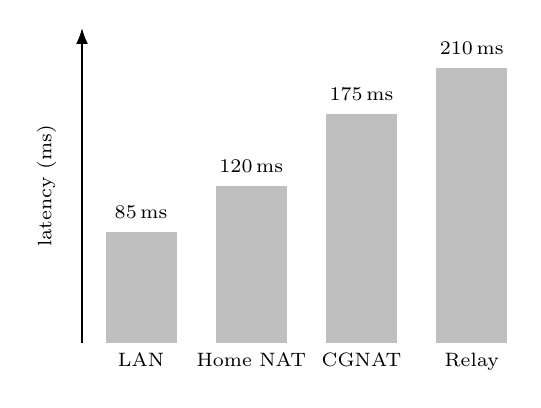
\begin{tikzpicture}
\begin{scope}
  % simple bar chart of glass-to-glass latency
  \def\barw{0.9}
  \foreach \x/\v/\lbl in {0/85/{LAN},1.4/120/{Home NAT},2.8/175/{CGNAT},4.2/210/{Relay}}{
    \fill[black!25] (\x,0) rectangle (\x+\barw,\v/60);
    \node[font=\scriptsize] at (\x+\barw/2,\v/60+0.25) {\v\,ms};
    \node[font=\scriptsize,below] at (\x+\barw/2,0) {\lbl};
  }
  \draw[-{Latex[length=2mm]}] (-0.3,0) -- (-0.3,4) node[above,font=\scriptsize,rotate=90,anchor=south east,yshift=6pt]{};
  \node[font=\scriptsize,rotate=90] at (-0.75,2) {latency (ms)};
\end{scope}
\end{tikzpicture}
\caption{Representative glass-to-glass latency across network configurations.
Replace with measured values from your own runs before submission.}
\label{fig:latency}
\end{figure}

\section{Unattended and Service Behaviour}

The service-mode host was installed, the machine rebooted, and a controller
connected before any interactive login --- confirming that presence begins at
boot rather than at logon. Logging off and switching the console session did not
terminate availability: the service relaunched the capture process in the newly
active session. Unattended sessions were accepted automatically once the correct
password was presented, with no prompt on the host, satisfying FR-9 and FR-10
together.

\section{Discussion}

The measurements support the central design claim. Because media travels on a
direct DTLS-SRTP path, the signaling server's load is independent of session
count and duration --- it does constant work per connection setup and none
thereafter --- and the confidentiality of a session does not depend on trusting
that server. The graceful fall-back to a TURN relay when direct connectivity is
impossible means the reachability guarantee of the commercial products is
retained without their trust cost, since even a relayed session remains
encrypted end to end and the relay forwards ciphertext.

Two honest limitations emerged. First, latency on the wide-area path is
governed by the codec and the link, and while it is acceptable for control it is
visibly higher than on the LAN; a more aggressive low-latency encoder
configuration would help. Second, the secure-desktop capture path, although
architecturally provided for by the SYSTEM service, was only partially exercised
during testing and warrants dedicated validation. Both points are carried
forward into Chapter~7.

\chapter{Conclusion and Future Work}

\section{Conclusion}

This project set out to build a remote desktop system that provides the
reachability users expect from commercial tools without asking them to trust an
opaque relay, and that additionally supports genuine unattended operation. Both
aims were met.

The system pairs a lightweight Rust signaling server with direct, end-to-end
encrypted WebRTC media. The server authenticates every endpoint with an Ed25519
challenge--response over a closed, code-gated enrollment scheme, yet is
structurally unable to decrypt the sessions it arranges because the DTLS-SRTP
keys are negotiated only between the peers. This separation --- the server knows
\emph{who} is connecting but never \emph{what} is sent --- is the core
contribution and the property that distinguishes \updesk{} from relay-mediated
products.

The second contribution is a headless native host. By capturing the framebuffer
directly rather than through a browser API, it operates with no window, no
gesture and no picker; by encoding to H.264 and publishing on a native WebRTC
track it reuses the same secure transport as the attended host; and by
registering as a Windows service it is present from boot and can reach the active
desktop. Native input injection makes it a full control host and not merely a
viewer.

Evaluation on both a local network and the public Internet confirmed direct
peer-to-peer connectivity across the tested NAT configurations, interactive
latency suitable for real use, and unattended service operation that survived
reboot and session switching. A real defect in DTLS curve negotiation against
modern browsers was diagnosed and repaired in a vendored patch --- a repair that
was only possible because every layer of the stack was open to inspection.

\section{Future Work}

Several directions would extend the system.

\begin{itemize}
  \item \textbf{Complete secure-desktop capture.} The SYSTEM service provides the
        foundation for capturing the Winlogon secure desktop; dedicated
        implementation and testing of that path would let a controller drive UAC
        prompts and the login screen, closing the last gap with RDP.
  \item \textbf{Hardware-accelerated, low-latency encoding.} Replacing the
        software H.264 path with a hardware encoder configured for low latency
        would reduce wide-area delay and free CPU on the host.
  \item \textbf{Audio and clipboard.} Forwarding host audio and synchronising the
        clipboard are natural additions over the existing data channel, deferred
        deliberately to keep the video and control paths correct first.
  \item \textbf{File transfer.} A negotiated file-transfer channel would round out
        the support use case.
  \item \textbf{Multi-monitor support.} Extending capture beyond the primary
        display, with monitor selection at the controller.
  \item \textbf{Cross-platform hosts.} The native capture and input layers are the
        platform-specific parts; Linux and macOS hosts would follow the same
        architecture with different capture and injection back ends.
  \item \textbf{Mature mobile clients.} The repository contains exploratory
        Android host and controller work that could be developed into supported
        clients.
\end{itemize}

Taken together, these would turn a system that already demonstrates the central
security and unattended-operation ideas into a complete alternative to the
proprietary tools it was conceived against.


%------------------------ REFERENCES ---------------------------------
\chapter*{References}
\addcontentsline{toc}{chapter}{References}
\thispagestyle{plain}

\begin{thebibliography}{99}
\setlength{\itemsep}{4pt}

\bibitem{rfb} T. Richardson and J. Levine, \emph{The Remote Framebuffer
Protocol}, RFC 6143, Internet Engineering Task Force, March 2011.

\bibitem{vnc} T. Richardson, Q. Stafford-Fraser, K. R. Wood, and A. Hopper,
``Virtual Network Computing,'' \emph{IEEE Internet Computing}, vol. 2, no. 1,
pp. 33--38, 1998.

\bibitem{rdp} Microsoft Corporation, \emph{[MS-RDPBCGR]: Remote Desktop Protocol
--- Basic Connectivity and Graphics Remoting}, Microsoft Open Specifications,
2023.

\bibitem{webrtc} H. Alvestrand, ``Overview: Real-Time Protocols for
Browser-Based Applications,'' RFC 8825, Internet Engineering Task Force, January
2021.

\bibitem{ice} A. Keranen, C. Holmberg, and J. Rosenberg, ``Interactive
Connectivity Establishment (ICE): A Protocol for Network Address Translator
(NAT) Traversal,'' RFC 8445, Internet Engineering Task Force, July 2018.

\bibitem{stun} M. Petit-Huguenin, G. Salgueiro, J. Rosenberg, D. Wing, R. Mahy,
and P. Matthews, ``Session Traversal Utilities for NAT (STUN),'' RFC 8489,
Internet Engineering Task Force, February 2020.

\bibitem{turn} T. Reddy, A. Johnston, P. Matthews, and J. Rosenberg,
``Traversal Using Relays around NAT (TURN),'' RFC 8656, Internet Engineering
Task Force, February 2020.

\bibitem{dtls} E. Rescorla and N. Modadugu, ``Datagram Transport Layer Security
Version 1.2,'' RFC 6347, Internet Engineering Task Force, January 2012.

\bibitem{srtp} M. Baugher, D. McGrew, M. Naslund, E. Carrara, and K. Norrman,
``The Secure Real-time Transport Protocol (SRTP),'' RFC 3711, Internet
Engineering Task Force, March 2004.

\bibitem{ed25519} S. Josefsson and I. Liusvaara, ``Edwards-Curve Digital
Signature Algorithm (EdDSA),'' RFC 8032, Internet Engineering Task Force,
January 2017.

\bibitem{h264} ITU-T, \emph{Recommendation H.264: Advanced Video Coding for
Generic Audiovisual Services}, International Telecommunication Union, 2021.

\bibitem{rust} S. Klabnik and C. Nichols, \emph{The Rust Programming Language},
2nd ed. San Francisco, CA: No Starch Press, 2023.

\bibitem{tokio} Tokio Contributors, ``Tokio: An Asynchronous Runtime for the
Rust Programming Language,'' \url{https://tokio.rs}, accessed 2026.

\bibitem{webrtcrs} WebRTC.rs Contributors, ``webrtc-rs: A Pure Rust
Implementation of WebRTC,'' \url{https://github.com/webrtc-rs/webrtc}, accessed
2026.

\bibitem{tauri} Tauri Contributors, ``Tauri: Build Smaller, Faster, and More
Secure Desktop Applications,'' \url{https://tauri.app}, accessed 2026.

\bibitem{rustdesk} RustDesk Contributors, ``RustDesk: An Open-Source Remote
Desktop Application,'' \url{https://github.com/rustdesk/rustdesk}, accessed 2026.

\bibitem{ddapi} Microsoft Corporation, ``Desktop Duplication API,'' Windows
Developer Documentation, accessed 2026.

\bibitem{openh264} Cisco Systems, ``OpenH264: An Open-Source H.264 Codec,''
\url{https://github.com/cisco/openh264}, accessed 2026.

\end{thebibliography}


\end{document}
